\documentclass[letterpaper, 12pt]{article}

\usepackage[utf8]{inputenc}
\usepackage[english, spanish]{babel}
\usepackage{fullpage}
\usepackage{graphicx}
\usepackage{amsmath}
\usepackage{enumitem}
\usepackage{chngcntr}
\usepackage{setspace}
\usepackage{url}
\usepackage{csquotes}
\usepackage{float}
\usepackage{verbatim}
\usepackage{tabularx}
\usepackage{amsmath}

\counterwithin{figure}{section}
\renewcommand{\thesection}{\arabic{section}}
\renewcommand{\thesubsection}{\thesection.\arabic{subsection}}
\renewcommand{\baselinestretch}{1.5}

\usepackage[style=apa, maxnames=6, minnames=3, backend=biber]{biblatex}
\DefineBibliographyStrings{english}{%chktex-file 1 chktex-file 6
	andothers = {\em et\addabbrvspace al\adddot}
}
\addbibresource{./Bibliography/bibliography.bib}

\usepackage{array}
\usepackage{enumitem}

\setlength{\parskip}{0pt}

\raggedbottom{}

\begin{document}

\begin{titlepage}
	\centering
	
\includegraphics[width=0.3\textwidth]{Images/logo_utb.png}\par\vspace{1cm}
	{\scshape\LARGE Universidad Tecnológica de Bolívar \par}
	\vspace{1cm}

	{\scshape\Large FÍSICA ELÉCTRICA \par}
	\vspace{.2cm}

	% chktex-file 8
	{\scshape\Large M2 - C \par}
	\vspace{1cm}
	% chktex-file 8
	\slshape {\Large \bfseries{}Informe de Laboratorio No. V\\}
	\vspace{1cm}

	\slshape {\itshape{} Dina Marcela Valenzuela Acosta, T00067398 \\}
	\slshape {\itshape{} Zaray Johana Riaño Vargas, T0006174 \\}
	\slshape {\itshape{} Jorge Marin Navarro, T00066518 \\}
	\slshape {\itshape{} Sergio Guerrero Herrera, T00068199 \\}
	\vfill
	Revisado Por \\
	Gabriel Hoyos Gomez Casseres\\
	{\large \today\par}
\end{titlepage}

% ----------------------------------------------------------------------|>
\section{Introducción}

\nocite{magnetic-fields-khanacademy}
\nocite{kirchhoff}

A lo largo de la experiencia \#5 ``circuitos de corriente
eléctrica''. Leyes de Kirchhoff” vamos a realizar circuitos
(de forma práctica) para así lograr analizar y verificar
las leyes de Kirchhoff; para poder desarrollar este informe
fue necesario tener términos claros como lo son:
resistencia, capacitores, diferencias de potencial, cuales
son las leyes de Kirchhoff, entre otros. A lo largo del
desarrollo del informe vamos a observar cálculos como lo
son de diferencias de potencial, corrientes, para por medio
de estos resultados obtenidos poder sustentar las leyes de
Kirchhoff como lo son: la ley de mallas y ley de nodos.
Esto lo logramos realizar gracias a investigaciones
teóricas y lecciones teóricas previamente vistas y
realizadas
% ----------------------------------------------------------------------|>
\section{Objetivos}

\subsection{Objetivo general}

\begin{itemize}[label=$\triangleright$]
	\item -	Analizar los cálculos realizados y resultados obtenidos para así sustentar y comprobar las leyes de Kirchhoff.
\end{itemize}

\subsection{Objetivos específicos}

\begin{itemize}[label=$\triangleright$]
	\item Determinar cuantas y cuales son las leyes de Kirchhoff.
	\item Comprender el funcionamiento de un circuito eléctrico
	      (cuando este se encuentra en paralelo o en serie) y como
	      esto influye en el calculo del voltaje.
	\item Aplicar las leyes de Kirchhoff para calcular las corrientes
	      de un circuito.
\end{itemize}

% ----------------------------------------------------------------------|>
\section{Marco Teórico}

% -----------------------------------------------------------|>
\subsection{Corriente eléctrica}

Se llama corriente eléctrica al flujo de carga eléctrica a
traves de un material conductor, debido al desplazamiento
de los electrones que orbitan el núcleo de los átomos que
compo- nen al conductor. Este movimiento de partículas se
inicia una vez que en los extremos del conductor se aplica
una tension externa, como una batería, por ejemplo. Esta
tension genera un campo eléctrico sobre los electrones que,
al poseer carga negativa, se ven atraídos hacia la terminal
positiva.

\begin{equation}
	I = \frac{dQ}{dt}
\end{equation}

% -----------------------------------------------------------|>
\subsection{Leyes de Kirchhoff}

Las leyes de Kirchhoff consisten en aplicar el principio de
conservación de la carga eléctrica y el principio de
conservación de la energía a los circuitos eléctricos, con
la finalidad de resolver los que tienen varias mallas. Es
conveniente saber el significado de algunos conceptos
importantes sobre circuitos eléctricos:

\begin{itemize}[label=$\triangleright$]
	\item Nodo: punto de union entre dos o más alambres conductores.
	\item Malla: Trayectoria o lazo cerrado compuesto de dos o más
	      ramas y que se recorre en un mismo sentido, sin pasar dos
	      veces por el mismo punto.
\end{itemize}

% -----------------------------------------------------------|>
\subsubsection{Primera ley de Kirchhoff}

Es conocida también como ley de las corrientes o regla de
los nodos, y establece que: La suma de las corrientes que
entra a un nodo es igual a la suma de las corrientes que
salen de el. Así que, en forma matemática, la primera ley
se expresa como:

\begin{equation}
	\sum I = 0
\end{equation}

% -----------------------------------------------------------|>
\subsubsection{Segunda ley de Kirchhoff}

Otros nombres para la segunda ley de Kirchhoff son: ley de
los voltajes, ley de las tensiones o ley de las mallas. En
cualquier caso, establece que: La suma algebraica de las
caídas de tension a lo largo de una malla es igual a 0.
Esta es una forma de aplicar la conservación de la energía
en el circuito, ya que el voltaje en cada elemento es el
cambio de energía por unidad de carga. Por lo tanto, al
recorrer una porción cerrada (una malla), la suma
algebraica de las subidas y caídas de tension es 0 y se
puede escribir:

\begin{equation}
	\sum V = 0
\end{equation}

\begin{itemize}[label=$\triangleright$]
	\item Cuando la flecha apunta en sentido de a hacia b: \hfill
	      \break{} $V_b =$ El voltaje mas positivo $V_r = V_a - V_b$
	\item Cuando la flecha apunta en sentido de a hacia a: \hfill
	      \break{} $V_a =$ El voltaje mas positivo $V_r = V_b - V_a$
\end{itemize}

\begin{equation}
	\begin{gathered}
		I1 = \frac{Vbc}{R1}, \hspace*{.3cm}
		I2 = \frac{Vcd}{R2}, \hspace*{.3cm}
		I3 = \frac{Vef}{R3}, \hspace*{.3cm}
		I4 = \frac{Vhf}{R4}
	\end{gathered}
\end{equation}

% ----------------------------------------------------------------------|>
\section{Montaje Experimental}

Para la realización de este informe en el laboratorio
utilizamos los siguientes materiales para hacer el circuito
que nos servirá para comprobar las leyes de Kirchhoff:
Alambres conductores, multímetro digital, 2 fuentes de D.C,
4 resistores y 1 tablero DINP Luego armamos el siguiente
esquema haciendo uso de nuestros materiales:

\begin{figure}[H]
	\centering
	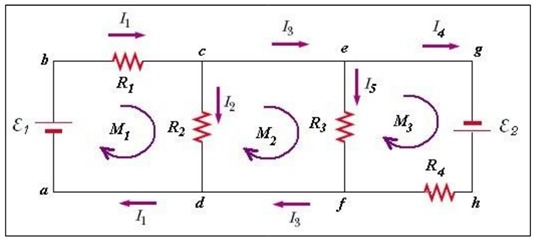
\includegraphics[scale = .5]{./Images/Imagen1.jpeg}
\end{figure}

Debemos tener en cuenta al momento de montar el circuito,
colocar en la salida de las fuentes un voltaje adecuado de
tal forma que los resistores puedan disipar la potencia que
se les entrega sin recalentarse ya que cuando se trabaja
con resistencias reales en el laboratorio el simulador no
tiene en cuenta que las resistencias se puedan fundir. En
la siguiente imagen podemos ver el montaje del circuito
hecho en el laboratorio:

\begin{figure}[H]
	\centering
	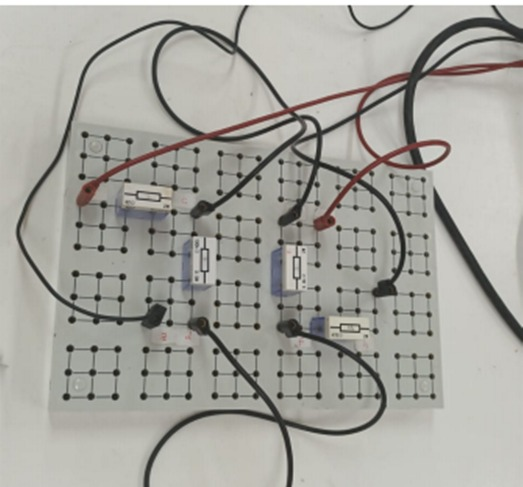
\includegraphics[scale = .5]{./Images/Imagen2.jpeg}
\end{figure}

% ----------------------------------------------------------------------|>
\section{Datos Experimentales}

% chktex-file 44
\begin{tabularx}{0.9\linewidth}{|>{\centering\arraybackslash}X|>{\centering\arraybackslash}X|>{\centering\arraybackslash}X|>{\centering\arraybackslash}X|}
	% \hline
	\multicolumn{4}{c}{Valor de resistencias $(\Omega)$} \\ \hline

	$R1$   & $R2$  & $R3$  & $R4$                        \\ \hline
	$1000$ & $330$ & $470$ & $2.2$                       \\ \hline
\end{tabularx}

\vspace{.5cm}

\begin{tabularx}{0.9\linewidth}{|>{\centering\arraybackslash}X|>{\centering\arraybackslash}X|>{\centering\arraybackslash}X|>{\centering\arraybackslash}X|>{\centering\arraybackslash}X|}
	% \hline
	\multicolumn{5}{c}{Valor de corrientes $(mA)$}  \\ \hline

	$I1$    & $I2$    & $I3$    & $I4$    & $I5$    \\ \hline
	$10.39$ & $10.39$ & $10.39$ & $10.39$ & $10.39$ \\ \hline
\end{tabularx}

\vspace{.5cm}

\begin{tabularx}{0.9\linewidth}{|>{\centering\arraybackslash}X|>{\centering\arraybackslash}X|>{\centering\arraybackslash}X|>{\centering\arraybackslash}X|>{\centering\arraybackslash}X|>{\centering\arraybackslash}X|>{\centering\arraybackslash}X|}
	% \hline
	\multicolumn{7}{c}{Diferencias de potencial $(V)$}                                    \\ \hline

	$E1 = B_{ab}$ & $V_{bc}$ & $V_{cd}$ & $V_{ef}$ & $E2 = V_{gh}$ & $V_{hf}$ & $V_{ce}$  \\ \hline
	$11.83$       & $-10.02$ & $-1.8$   & $-1.809$ & $0.0207$      & $-1.8$   & $-0.0002$ \\ \hline
\end{tabularx}

\vspace{.5cm}

\begin{tabularx}{0.9\linewidth}{|>{\centering\arraybackslash}X|>{\centering\arraybackslash}X|>{\centering\arraybackslash}X|>{\centering\arraybackslash}X|>{\centering\arraybackslash}X|}
	% \hline
	\multicolumn{5}{c}{Valor de corrientes [\textit{(FEM)} Invertida] $(mA)$} \\ \hline

	$I1$    & $I2$   & $I3$  & $I4$ & $I5$                                    \\ \hline
	$10.35$ & $5.76$ & $4.6$ & $4$  & $0.59$                                  \\ \hline

\end{tabularx}

% ----------------------------------------------------------------------|>
\section{Análisis de datos}

% -----------------------------------------------------------|>
\subsection{Sume las diferencias de potencial en cada uno de los elementos del circuito para cada
	malla. Registre sus cálculos en la tabla 5.}

% chktex-file 44
\begin{tabularx}{0.9\linewidth}{|>{\centering\arraybackslash}X|>{\centering\arraybackslash}X|}
	\hline

	\textbf{Malla} & \textbf{V}                                                                 \\ \hline
	$M1$           & $V_{ab} + V_{bc} + V_{cd} = 11.83V - 10.02V -1.8V = 0V$
	$11.83V \sim 11.82V$                                                                        \\ \hline

	$M2$           & $V_{dc} + V_{ef} = 1.8V - 1.809V = 0V$
	$1.8V \sim 1.809V$                                                                          \\ \hline

	$M3$           & $V_{gh} + V_{hf} + V_{fe} = 2.7mV - 1.81V + 1.809V = 0V$
	$1.8117V \sim 1.81V$                                                                        \\ \hline

	$A_{bgh}$      & $V_{ab} + V_{bg} + V_{gh} + V_{ha} = 11.83V - 10.02V + 2.7mV - 1.81V = 0V$
	$11.83V = 11.83V$                                                                           \\ \hline

	$A_{bef}$      & $V_{ab} + V_{be} + V_{ef} = 11.83V - 10.02V - 1.809V = 0V$
	$11.83V = 11.83V$                                                                           \\ \hline

	$C_{ghd}$      & $V_{cg} + V_{gh} + V_{hd} + V_{dc} = 0V + 2.7mV - 1.81V + 1.8V = 0V$
	$1.8V \sim 1.81V$                                                                           \\ \hline
\end{tabularx}

% -----------------------------------------------------------|>
\subsection{¿Se cumple la ley de las mallas? ¿por qué?}

Si se cumple la ley de malla, ya que los valores practico y
teóricos coinciden con un pequeño error debido a la
tolerancia de los elementos o la impresión del dispositivo
de medida.

% -----------------------------------------------------------|>
\subsection{¿Si no resulta lo que se espera, a qué se deberá?}

Si no resulta lo que se espera es producto de un error, ya
se una no adecuada medición, fallas del dispositivo o
errores de cálculos.

% -----------------------------------------------------------|>
\subsection{¿Si realiza el recorrido en sentido contrario, también se cumple
	la ley de las mallas? ¿Cuál es la diferencia?}

Si se cumple y la diferencia es que la corriente resultara
con signos contrario, igual magnitud, pero diferentes
signos.

% -----------------------------------------------------------|>
\subsection{¿Por qué Vce es cero?}

Porque es un cable y el diferencial es sus extremos es
igual, pero con diferentes signos

% -----------------------------------------------------------|>
\subsection{Sume las corrientes que salen en cada nodo. Registre sus datos en la tabla 6}

\begin{tabularx}{0.9\linewidth}{|>{\centering\arraybackslash}X|>{\centering\arraybackslash}X|>{\centering\arraybackslash}X|}
	\hline
	Nodo & Entra                                  & Sale                                  \\ \hline
	$C$  & $I1 = 10.35mA$                         & $I2 + I3 = 5.76mA + 4.60mA = 10.36mA$ \\ \hline
	$E$  & $I3 = 4.75mA$                          & $I4 + I5 = 3.92mA + 0.83mA = 4.75mA$  \\ \hline
	$D$  & $I4 + I5 = 3.92mA + 0.83mA = 4.75mA$   & $I3 = 4.75mA$                         \\ \hline
	$F$  & $I2 + I3 = 5.76mA + 4.60mA = 10.36mA $ & $I1 = 10.35mA $                       \\\hline
\end{tabularx}

% -----------------------------------------------------------|>
\subsection{¿Se cumple la ley de los nodos? ¿Por qué?}

Si se cumple, ya que la suma de todas las corrientes
medidas es igual a cero.

% -----------------------------------------------------------|>
\subsection{¿Si no resulta lo que se espera, a qué se deberá?}

Si no resulta lo que se espera es producto de un error, ya
se una no adecuada medición, fallas del dispositivo o
errores de cálculos.

% -----------------------------------------------------------|>
\subsection{Aplique las leyes de Kirchhoff para encontrar una expresión que nos permita calcular las
	corrientes en el circuito en términos de las resistencias y fem. Registre los resultados en
	la tabla 7}

% chktex-file 26
.
% -----------------------------------------------------------|>
\subsection{Calcule los valores de las corrientes remplazando en la expresión encontrada los valores
	de las resistencias y las fem (tabla 1 y 2). Registre los resultados en la tabla 7}

% chktex-file 26
.
% -----------------------------------------------------------|>
\subsection{Calcule la exactitud de la medida directa de las corrientes respecto a los valores teóricos
	encontrados por las leyes de Kirchhoff. Registre los resultados en la tabla 7. De una
	explicación a las causas de las diferencias en las medidas.}

(Los puntos 9,10,11 están resueltos en la tabla 7)

\footnote{Tabla 7}
\begin{tabularx}{0.9\linewidth}{|>{\centering\arraybackslash}X|>{\centering\arraybackslash}X|>{\centering\arraybackslash}X|>{\centering\arraybackslash}X|}
	\hline
	Expresión                & I $(mA)$ Valor Teorico & I $(mA)$ Valor Medido & Exactitud                                                    \\\hline
	$I1 = \frac{V_{bc}}{R1}$ & $10.02$                & $10.39$               & $1 - (\frac{10.39 - 10.02}{10.39 + 10.02}) \cdot 100 = 96\%$ \\ \hline
	$I2 = \frac{V_{cd}}{R2}$ & $5.45$                 & $5.63$                & $1 - (\frac{5.63 - 5.45}{5.63 + 5.45}) \cdot 100 = 97\%$     \\ \hline
	$I3 = I4 + I5$           & $7.77$                 & $4.75$                & $1 - (\frac{7.77 - 4.75}{4.75 + 7.77}) \cdot 100 = 76\%$     \\ \hline
	$I4 = I3 - I5$           & $0.9$                  & $3.92$                & $1 - (\frac{3.92 - 0.9}{0.9 + 3.92}) \cdot 100 = 37\%$       \\ \hline
	$I5 = \frac{V_{ef}}{R3}$ & $3.85$                 & $0.83$                & $1 - (\frac{3.85 - 0.83}{0.83 + 3.85}) \cdot 100 = 35\%$     \\\hline
\end{tabularx}

% -----------------------------------------------------------|>
\subsection{Realice los procedimientos del 9 al 11, pero considerando la \textit{(FEM)} E2 invertida y los datos de la tabla 4}

\begin{tabularx}{0.9\linewidth}{|>{\centering\arraybackslash}X|>{\centering\arraybackslash}X|>{\centering\arraybackslash}X|>{\centering\arraybackslash}X|}
	\hline
	Expresión                & I $(mA)$ Valor Teorico & I $(mA)$ Valor Medido & Exactitud                                                    \\\hline
	$I1 = \frac{V_{bc}}{R1}$ & $10.02$                & $10.39$               & $1 - (\frac{10.39 - 10.02}{10.39 + 10.02}) \cdot 100 = 96\%$ \\ \hline
	$I2 = \frac{V_{cd}}{R2}$ & $5.45$                 & $5.63$                & $1 - (\frac{5.63 - 5.45}{5.63 + 5.45}) \cdot 100 = 97\%$     \\ \hline
	$I3 = I4 + I5$           & $7.77$                 & $4.75$                & $1 - (\frac{7.77 - 4.75}{4.75 + 7.77}) \cdot 100 = 76\%$     \\ \hline
	$I4 = I3 - I5$           & $0.9$                  & $3.92$                & $1 - (\frac{3.92 - 0.9}{0.9 + 3.92}) \cdot 100 = 37\%$       \\ \hline
	$I5 = \frac{V_{ef}}{R3}$ & $3.85$                 & $0.83$                & $1 - (\frac{3.85 - 0.83}{0.83 + 3.85}) \cdot 100 = 35\%$     \\\hline
\end{tabularx}

% -----------------------------------------------------------|>
\subsection{Observe todas las medidas que cambian (corrientes y diferencias de potencial) respecto
	al circuito inicial y de una explicación}

Como se ha mencionado anteriormente, los valores de
corriente y diferencia de potencial pueden variar
dependiendo de si se obtienen a partir de la teoría o de
mediciones realizadas en el laboratorio. En este tipo de
experimentos, las mediciones pueden no ser completamente
precisas, lo que resulta en una pequeña variación en los
valores calculados. Al comparar los procedimientos para el
circuito normal y la inversión de la fem E2, encontramos
que los valores son completamente diferentes. Esto se debe
a que la posición de esta fem determina la corriente que
fluye a través del circuito, lo que afecta cada corriente
según su trayectoria con la fem posicionada de esa manera.

% -----------------------------------------------------------|>
\subsection{Realice conclusiones y observaciones}

Las leyes de Kirchhoff tienen una gran importancia en el
campo de la física eléctrica y, especialmente, en todas las
áreas que trabajan con circuitos eléctricos. Estas leyes
permiten una comprensión más profunda del comportamiento de
las corrientes eléctricas y los voltajes en dichos
sistemas. En esta ocasión, se realizó un experimento
mediante la construcción de un circuito eléctrico, donde se
midieron valores de resistencia, voltaje e intensidad
eléctrica con el objetivo de verificar estas leyes de
manera práctica.

Los resultados también se ajustaron de manera
satisfactoria, tal como se puede apreciar en las tablas
correspondientes. La corriente que ingresa a cada nodo es
casi equivalente a la corriente que sale de ellos, lo cual
concuerda con lo establecido por la ley de Kirchhoff para
los nodos. En conclusión, los resultados obtenidos en la
práctica de laboratorio fueron precisos. Esto se evidencia
en la comparación entre los datos medidos y los datos
esperados, donde se muestra una alta exactitud. De esta
manera, los valores medidos experimentalmente siguen lo
planteado por la teoría, lo que permitió llevar a cabo y
concluir de manera adecuada la presente experiencia de
laboratorio relacionada con las leyes de Kirchhoff.

% ----------------------------------------------------------------------|>
\section{Conclusiones}

A lo largo del informe “circuitos de corriente eléctrica.
Leyes de Kirchhoff” logramos analizar, determinar,
comprender aplicar y explicar las leyes de Kirchhoff como
lo son la ley de las mallas y la ley de los nodos. En el
desarrollo del informe observamos que la diferencia de
potencial en un circuito va a depender de la trayectoria
que esta haga y de si el circuito se encuentra en serie o
en paralelo; también que cuando intercambiamos el circuito
de salida de una de las dos fem las corrientes varían en
algunos casos como se observa en las tablas aumenta o
disminuye; por medio de las leyes de Kirchhoff podemos
encontrar expresiones para calcular las corrientes del
circuito, Podemos concluir que las leyes de Kirchhoff
proporcionan una base sólida para el análisis y el diseño
de distintos tipos de circuitos.

\printbibliography

\end{document}